\chapter{Additional Results} \label{chap:Appendix}
\section{Classical Model}
\label{sec:ClassicalModel}
\subsection{Classification Result}
\begin{table}[H]
        \begin{center}
                \begin{tabular}{|l||c|c|c|c|}
                        \hline 
                        Evaluation metrics & Base & Translation & Rotation & Average \\
                        \hline \hline
                        Accuracy & 0.812 & 1 & 0.768 & 0.853 \\
                        \hline
                        Precision & 0.910 & 0.718 & 1 & 0.879 \\
                        \hline
                        Recall & 0.812 & 1 & 0.768 & 0.853 \\
                        \hline
                        f1-Score & 0.858 & 0.836 & 0.869 & 0.855 \\
                        \hline
                \end{tabular}
        \end{center}
        \caption{Classification results with the Classical model}
\end{table}
\subsection{Segmentation Result}
\begin{table}[H]
        \begin{center}
                \begin{tabular}{|l||c|c|c|}
                        \hline 
                         & Predicted base & Predicted translation & Predicted rotation \\
                        \hline \hline
                        Actual base & 0.812 & 0.188 & 0 \\
                        \hline
                        Actual translation & 0 & 1 & 0 \\
                        \hline
                        Actual rotation & 0.146 & 0.085 & 0.768 \\
                        \hline
                \end{tabular}
        \end{center}
        \caption{Segmentation results with the Classical model}
\end{table}
\section{Deep Learning Model}
\label{sec:DLModel}
\subsection{Classification Results}
\subsubsection{Case 1: Point cloud data without noise and theoretical flows}
\begin{table}[H]
        \begin{center}
                \begin{tabular}{|l||c|c|c|c|}
                        \hline 
                        Evaluation metrics & Base & Translation & Rotation & Average \\
                        \hline \hline
                        Accuracy  & 1.000 & 1.000 &  1.000 &  1.000\\
                        \hline
                        Precision & 1.000 &  1.000 &  1.000 &  1.000\\
                        \hline
                        Recall & 1.000&  1.000& 1.000 & 1.000 \\
                        \hline
                        f1-Score &  1.000&  1.000 & 1.000 & 1.000 \\
                        \hline
                \end{tabular}
        \end{center}
        \caption{Case 1 - Classification: Best model after 50 epochs. Obtained at epoch 36/50.}
\end{table}
\begin{figure}[H]
    \begin{subfigure}{.48\linewidth}
    \centering
    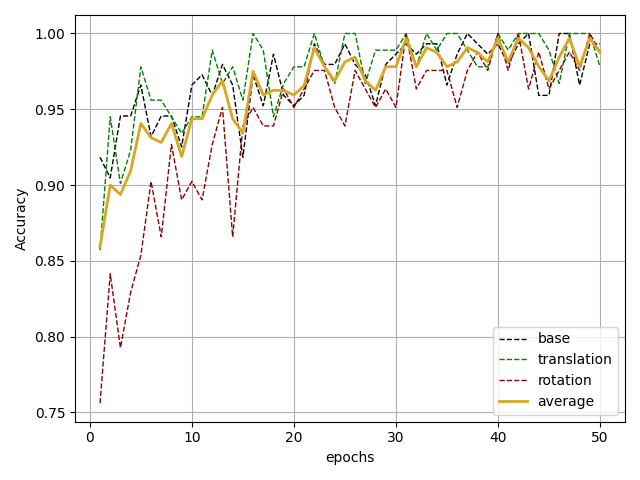
\includegraphics[scale=0.45]{Img/cls_nonoise_train_acc.png}
    \caption{Train}
    \end{subfigure}
    \begin{subfigure}{.48\linewidth}
    \centering
    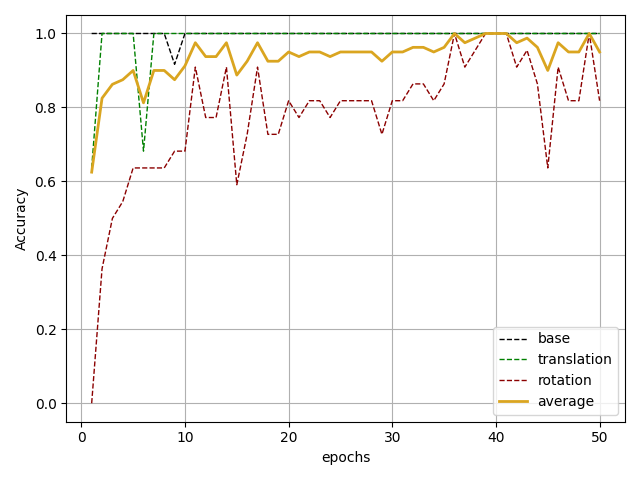
\includegraphics[scale=0.45]{Img/cls_nonoise_test_acc.png}
    \caption{Test}
    \end{subfigure}\\
    \caption{Case 1 - Classification: Accuracy metric. }
\end{figure}
\begin{figure}[H]
    \begin{subfigure}{.48\linewidth}
    \centering
    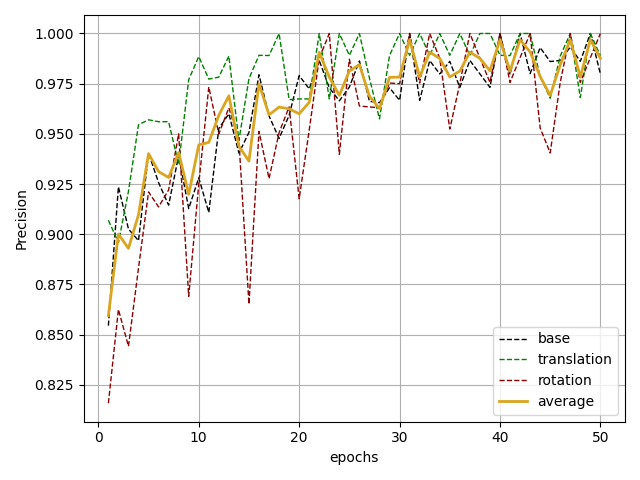
\includegraphics[scale=0.45]{Img/cls_nonoise_train_prec.png}
    \caption{Train}
    \end{subfigure}
    \begin{subfigure}{.48\linewidth}
    \centering
    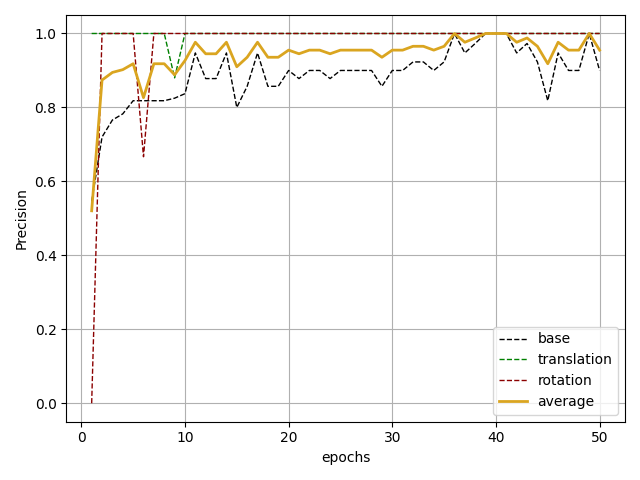
\includegraphics[scale=0.45]{Img/cls_nonoise_test_prec.png}
    \caption{Test}
    \end{subfigure}\\
    \caption{Case 1 - Classification: Precision metric.}
\end{figure}
\begin{figure}[H]
    \begin{subfigure}{.48\linewidth}
    \centering
    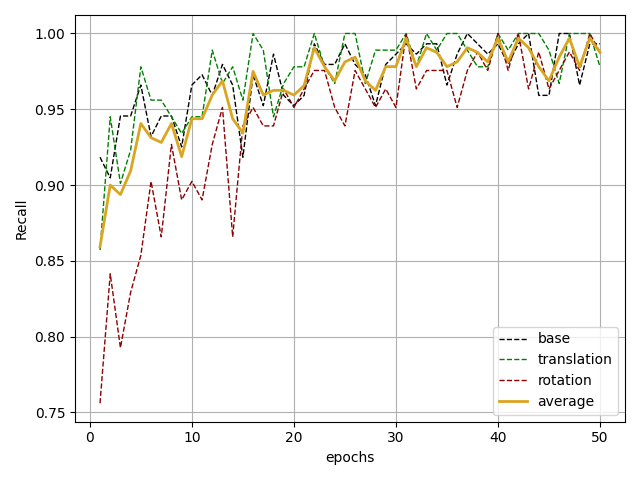
\includegraphics[scale=0.45]{Img/cls_nonoise_train_rec.png}
    \caption{Train}
    \end{subfigure}
    \begin{subfigure}{.48\linewidth}
    \centering
    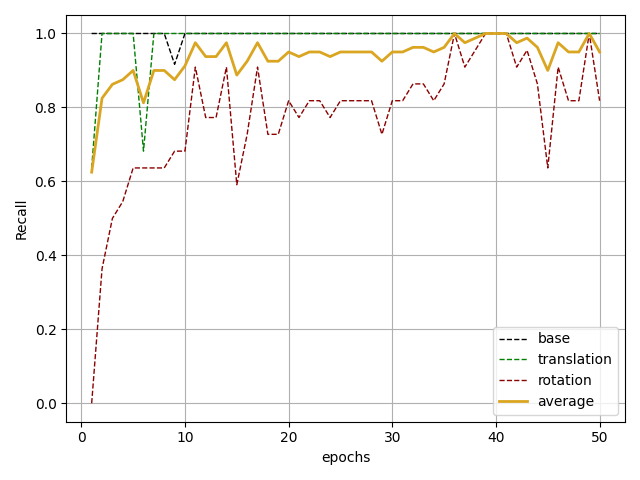
\includegraphics[scale=0.45]{Img/cls_nonoise_test_rec.png}
    \caption{Test}
    \end{subfigure}\\
    \caption{Case 1 - Classification: recall metric. }
\end{figure}
\begin{figure}[H]
    \begin{subfigure}{.48\linewidth}
    \centering
    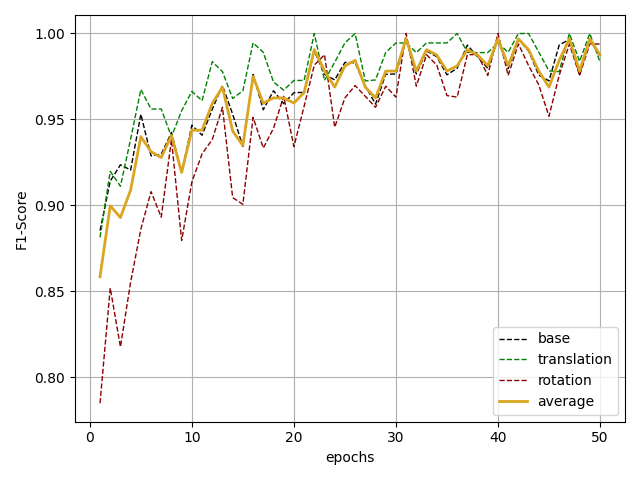
\includegraphics[scale=0.45]{Img/cls_nonoise_train_f1.png}
    \caption{Train}
    \end{subfigure}
    \begin{subfigure}{.48\linewidth}
    \centering
    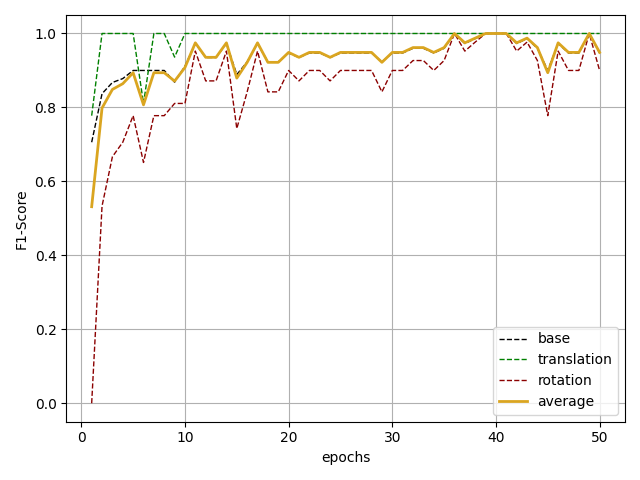
\includegraphics[scale=0.45]{Img/cls_nonoise_test_f1.png}
    \caption{Test}
    \end{subfigure}\\
    \caption{Case 1 - Classification: F1-score metric. }
\end{figure}
\subsubsection{Case 3: Point cloud data without noise and pre-trained flows}
\begin{table}[H]
        \begin{center}
                \begin{tabular}{|l||c|c|c|c|}
                        \hline 
                        Evaluation metrics & Base & Translation & Rotation & Average \\
                        \hline \hline
                        Accuracy  & 1.000 & 1.000 &  0.565 &  0.875\\
                        \hline
                        Precision & 0.756 &  1.000 &  1.000 &  0.905\\
                        \hline
                        Recall & 1.000&  1.000& 0.565 & 0.875 \\
                        \hline
                        f1-Score &  0.861&  1.000 & 0.722 & 0.866 \\
                        \hline
                \end{tabular}
        \end{center}
        \caption{Case 3 - Classification: Best model after 50 epochs. Obtained at epoch 36/50.}
\end{table}
\begin{figure}[H]
    \begin{subfigure}{.48\linewidth}
    \centering
    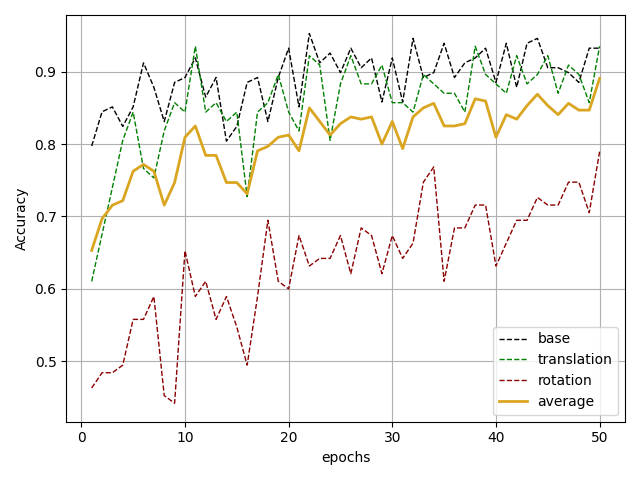
\includegraphics[scale=0.45]{Img/cls_flow_nonoise_train_acc.png}
    \caption{Train}
    \end{subfigure}
    \begin{subfigure}{.48\linewidth}
    \centering
    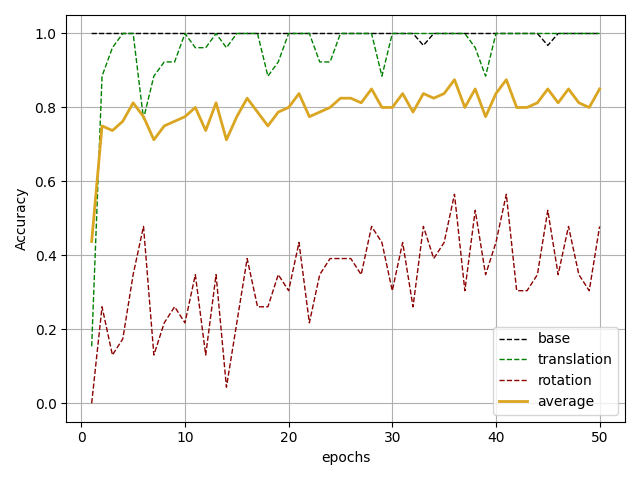
\includegraphics[scale=0.45]{Img/cls_flow_nonoise_test_acc.png}
    \caption{Test}
    \end{subfigure}\\
    \caption{Case 3 - Classification: Accuracy metric. }
\end{figure}
\begin{figure}[H]
    \begin{subfigure}{.48\linewidth}
    \centering
    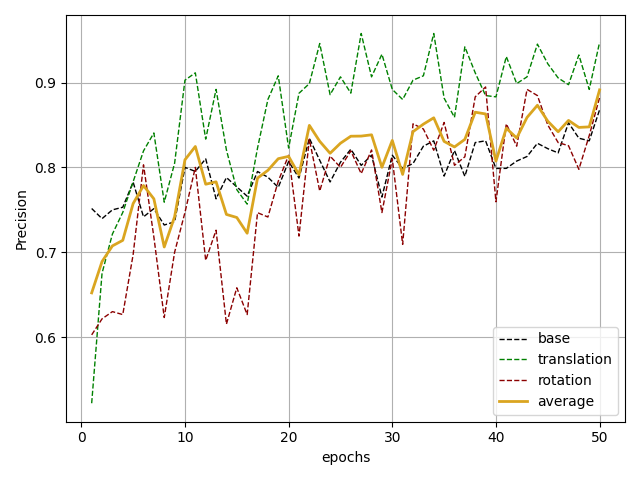
\includegraphics[scale=0.45]{Img/cls_flow_nonoise_train_prec.png}
    \caption{Train}
    \end{subfigure}
    \begin{subfigure}{.48\linewidth}
    \centering
    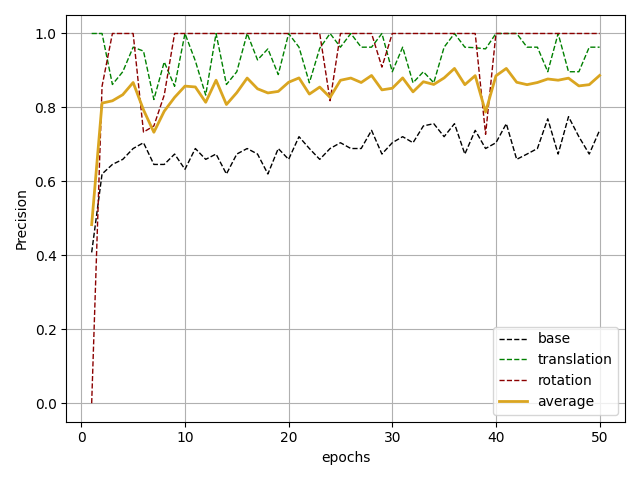
\includegraphics[scale=0.45]{Img/cls_flow_nonoise_test_prec.png}
    \caption{Test}
    \end{subfigure}\\
    \caption{Case 3 - Classification: Precision metric.}
\end{figure}
\begin{figure}[H]
    \begin{subfigure}{.48\linewidth}
    \centering
    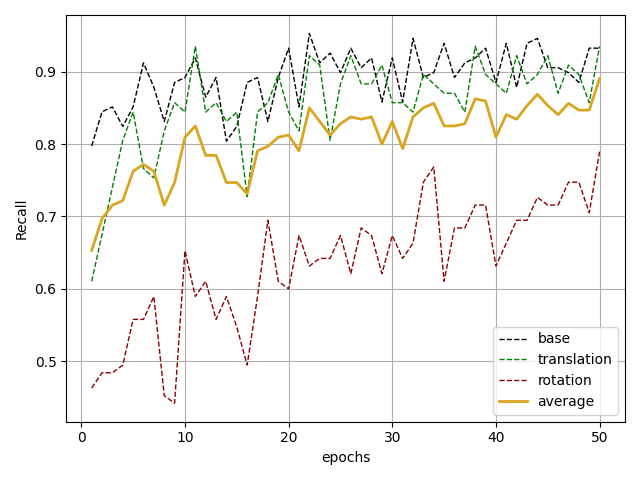
\includegraphics[scale=0.45]{Img/cls_flow_nonoise_train_rec.png}
    \caption{Train}
    \end{subfigure}
    \begin{subfigure}{.48\linewidth}
    \centering
    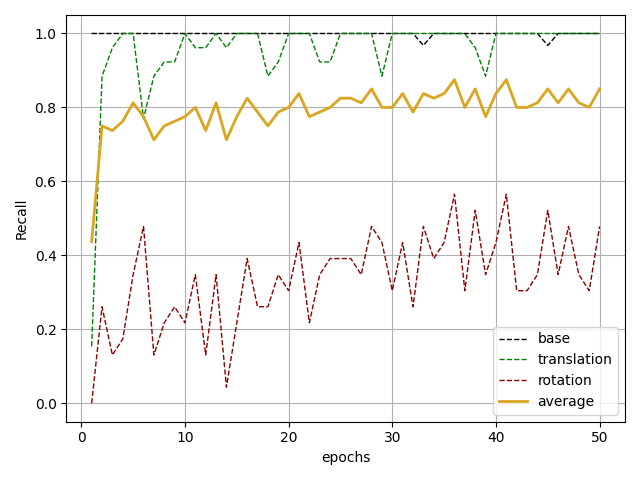
\includegraphics[scale=0.45]{Img/cls_flow_nonoise_test_rec.png}
    \caption{Test}
    \end{subfigure}\\
    \caption{Case 3 - Classification: Recall metric}
\end{figure}
\begin{figure}[H]
    \begin{subfigure}{.48\linewidth}
    \centering
    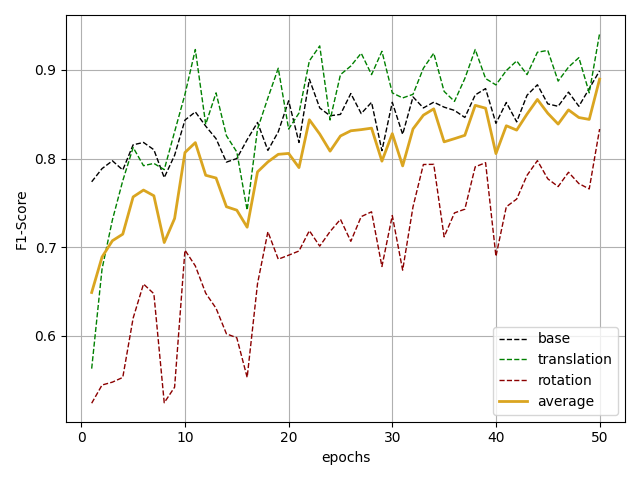
\includegraphics[scale=0.45]{Img/cls_flow_nonoise_train_f1.png}
    \caption{Train}
    \end{subfigure}
    \begin{subfigure}{.48\linewidth}
    \centering
    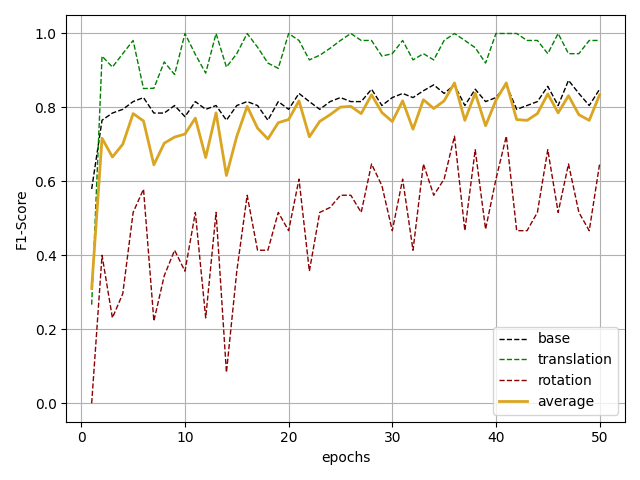
\includegraphics[scale=0.45]{Img/cls_flow_nonoise_test_f1.png}
    \caption{Test}
    \end{subfigure}\\
    \caption{Case 3 - Classification: F1-score metric}
\end{figure}



\subsection{Segmentation Results}
\subsubsection{Case 1: Point cloud data without noise and theoretical flows}
\begin{table}[H]
    \begin{center}
        \begin{tabular}{|l||c|c|c|c|}
            \hline
            Evaluation metrics & Base & Translation & Rotation & Average \\
            \hline \hline
            train accuracy & 0.967 & 0.965 & 0.796 & 0.910 \\
            \hline
            train IoU & 0.927 & 0.865 & 0.728 & 0.840 \\
            \hline
            test accuracy & 0.976 & 0.952 & 0.884 & 0.937 \\
            \hline
            test IoU & 0.951 & 0.894 & 0.809 & 0.884 \\
            \hline
        \end{tabular}
    \end{center}
    \caption{Case 1 - Segmentation: Best model after 50 epochs. Obtained at epoch 47/50.}
\end{table}
\begin{figure}[H]
    \begin{subfigure}{.48\linewidth}
    \centering
    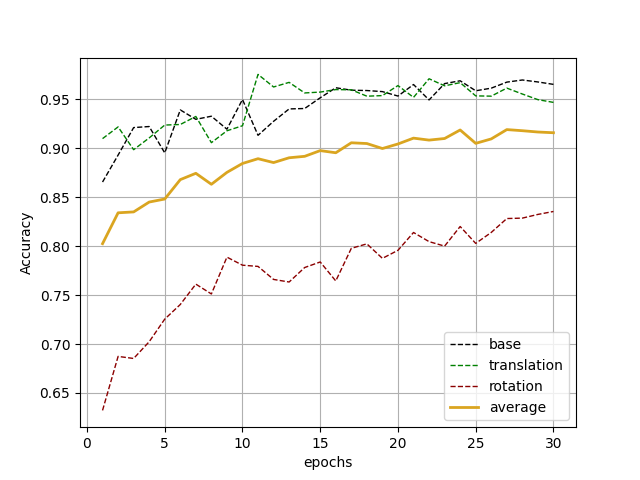
\includegraphics[scale=0.45]{Img/seg_nonoise_train_acc.png}
    \caption{Train}
    \end{subfigure}
    \begin{subfigure}{.48\linewidth}
    \centering
    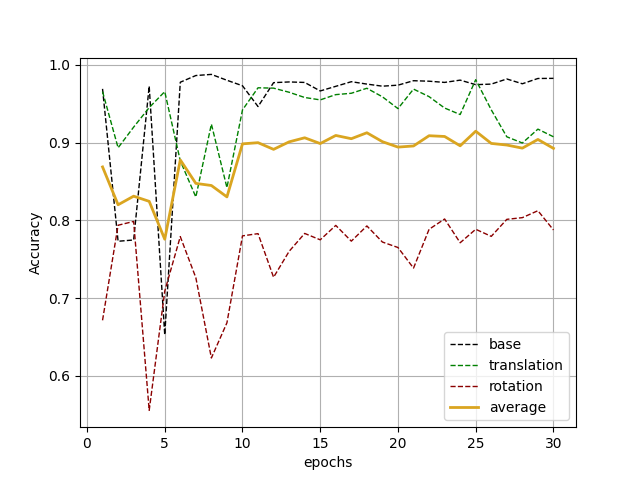
\includegraphics[scale=0.45]{Img/seg_nonoise_test_acc.png}
    \caption{Test}
    \end{subfigure}\\
    \caption{Case 1 - Segmentation: Accuracy metric.}
\end{figure}
\begin{figure}[H]
    \begin{subfigure}{.48\linewidth}
    \centering
    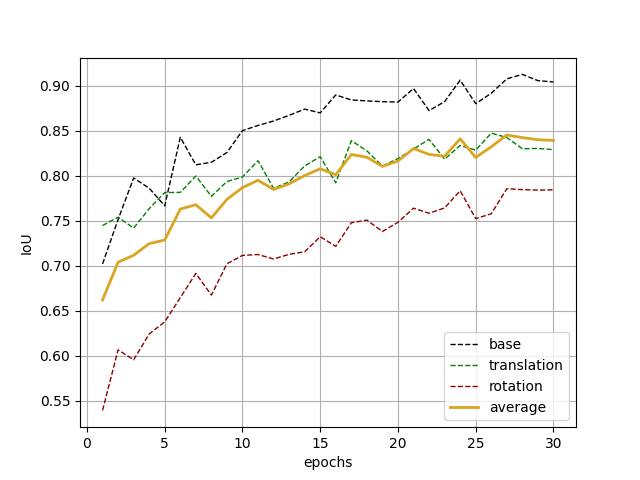
\includegraphics[scale=0.45]{Img/seg_nonoise_train_iou.png}
    \caption{Train}
    \end{subfigure}
    \begin{subfigure}{.48\linewidth}
    \centering
    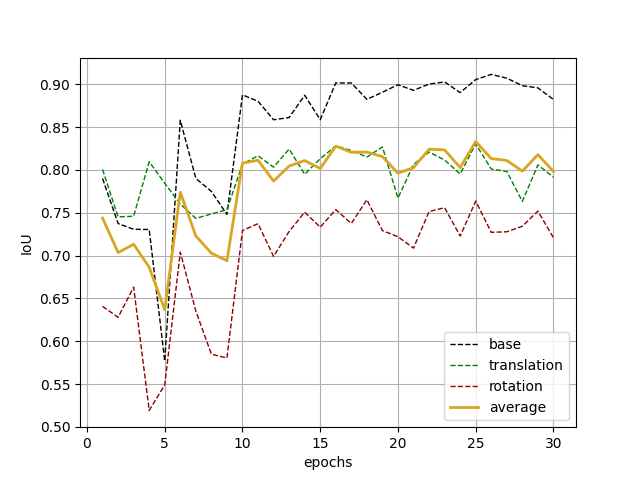
\includegraphics[scale=0.45]{Img/seg_nonoise_test_iou.png}
    \caption{Test}
    \end{subfigure}\\
    \caption{Case 1 - Segmentation: IoU metric.}
\end{figure}
\subsubsection{Case 3: Point cloud data without noise and pretrained flows}
\begin{table}[H]
    \begin{center}
        \begin{tabular}{|l||c|c|c|c|}
            \hline
            Evaluation metrics & Base & Translation & Rotation & Average \\
            \hline \hline
            train accuracy & 0.588 & 0.680 & 0.187 & 0.485 \\
            \hline
            train IoU & 0.352 & 0.419 & 0.145 & 0.305 \\
            \hline
            test accuracy & 0.613 & 0.666 & 0.208 & 0.496 \\
            \hline
            test IoU & 0.385 & 0.429 & 0.154 & 0.323 \\
            \hline
        \end{tabular}
    \end{center}
    \caption{Case 3 - Segmentation: Best model after 50 epochs. Obtained at epoch 42/50.}
\end{table}
\begin{figure}[H]
    \begin{subfigure}{.48\linewidth}
    \centering
    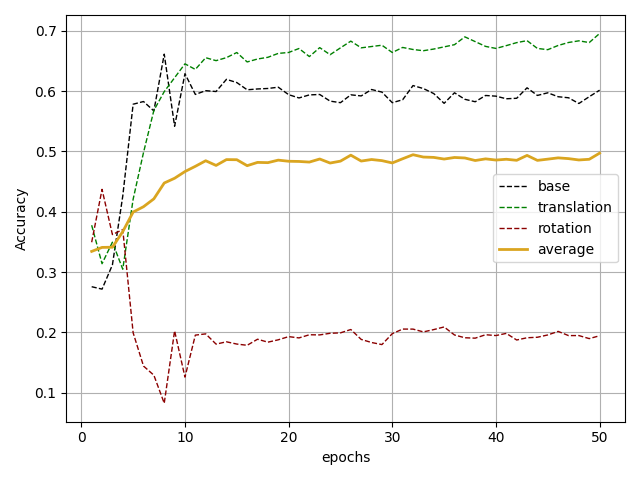
\includegraphics[scale=0.45]{Img/seg_flow_nonoise_train_acc.png}
    \caption{Train}
    \end{subfigure}
    \begin{subfigure}{.48\linewidth}
    \centering
    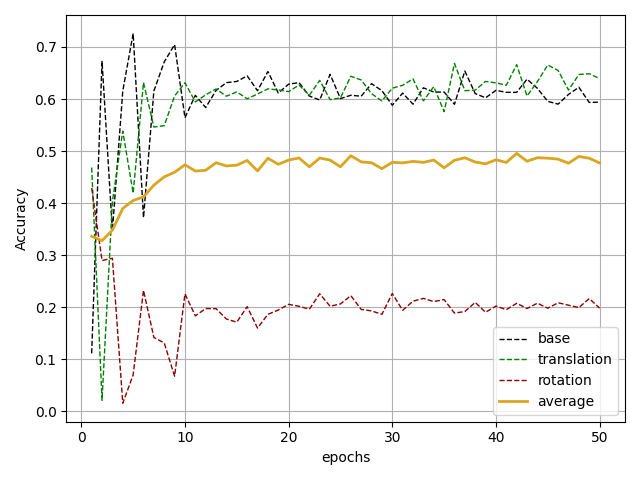
\includegraphics[scale=0.45]{Img/seg_flow_nonoise_test_acc.png}
    \caption{Test}
    \end{subfigure}\\
    \caption{Case 3 - Segmentation: Accuracy metric.}
\end{figure}
\begin{figure}[H]
    \begin{subfigure}{.48\linewidth}
    \centering
    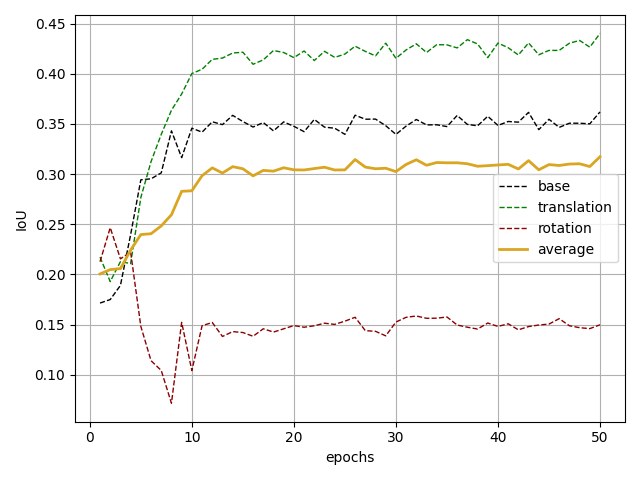
\includegraphics[scale=0.45]{Img/seg_flow_nonoise_train_iou.png}
    \caption{Train}
    \end{subfigure}
    \begin{subfigure}{.48\linewidth}
    \centering
    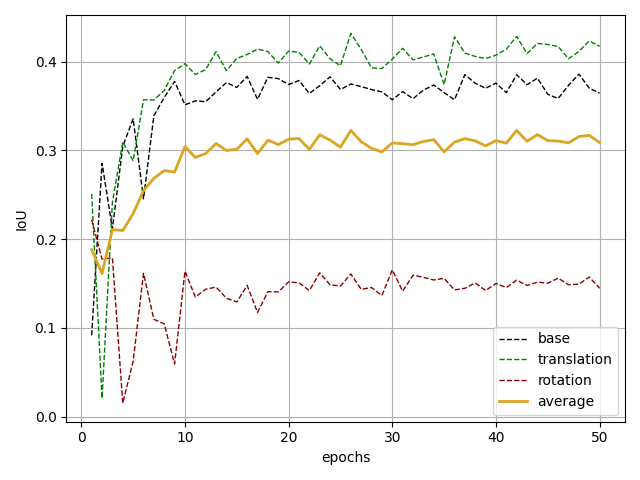
\includegraphics[scale=0.45]{Img/seg_flow_nonoise_test_iou.png}
    \caption{Test}
    \end{subfigure}\\
    \caption{Case 3 - Segmentation: IoU metric.}
\end{figure}